\documentclass[12pt,a4paper]{article}
\usepackage[utf8]{inputenc}
\usepackage[T1]{fontenc}
\usepackage{amsmath}
\usepackage{amsfonts}
\usepackage[francais]{babel}
\usepackage{amssymb}
\usepackage{graphicx}
\usepackage[top=2.00cm]{geometry}
\usepackage{enumitem}
\usepackage{tikz}
\usepackage{mathtools}
\usepackage{pgfplots}
\usetikzlibrary{plotmarks}
\usepackage{bigcenter}
\usepackage{multicol}
\date{3 novembre 2016}
%Modif des enumerates numeros en gras. leftmargin=*,
\setlist[enumerate]{label=\textbf{\arabic*}.}

\usepackage{titlesec}
%modif des titres de section diminuer la taille
\titleformat{\section}
  {\normalfont\fontsize{14}{15}\bfseries}{\thesection}{1em}{}
\titleformat{\subsection}
  {\normalfont\fontsize{12}{15}\bfseries}{\thesubsection}{1em}{}


\author{CHARNAY Valentin, FINOT Sylvain}
\title{Compte rendu de TP : \\ Régulation de tension}

\begin{document}
\maketitle
L'objectif de ce TP est de comparer différents montages permettant d'obtenir une tension continue à partir d'alternatif.
\section{Redressement et filtrage}
%\subsection{Étude du montage à basse fréquence (Amplificateur Opérationnel considéré idéal)}
\begin{enumerate}
\item Nous cherchons à obtenir un signal continu à partir d'un générateur de tension alternatif 7V. Pour ce faire nous utilisons un pont de diodes (pont de Graëtz) qui permet dans un premier temps de redresser la partie négative du signal. Le signal ressemble alors à la valeur absolue d'une sinusoïde. Cependant nous cherchons a obtenir un signal continu. Il suffit alors de mettre un condensateur en parallèle, celui ci va jouer le rôle de réservoir ("buffer"), permettant ainsi d'obtenir un signal relativement continu/stable. Cela veut donc dire que ce montage marche bien lorsque l'utilisateur ne demande pas trop de courant et donc que la décharge du condensateur est minime $\implies$ $R_{c}$(résistance simulant l'utilisateur) très grande.\\
Une fois le montage réalisé, on peut être tenté de regarder simultanément sur l'oscilloscope le signal en sortie du générateur et le signal au bornes du condensateur. C'est une très mauvaise idée, cela reviendrait a court-circuiter une des diodes du pont puisque deux de ses bornes seraient reliés au même point, la masse de l'oscilloscope.

\item On observe par la suite la différence entre le signal de sortie avec R$_{c}$=1k$\Omega$ et sans R$_{c}$ $\iff$ R$_{c}=+ \infty$. On remarque que le taux d'ondulation : \[T\equiv \dfrac{\delta V}{V} \] est beaucoup plus important lorsque R$_{c}=1$k$\Omega$. \\
On essaye alors de mesurer T avec précision, on regarde d'abord la tension de sortie puis uniquement le taux d'ondulation.
\begin{multicols}{2}
\begin{itemize}
\item Pour R$_{c}=+ \infty$ :\\
% Pas sur du calibre pour T
U$_{s}=10\pm1$V \\
$\delta U_{s}$=0,2mV (calibre 1mV/div)\\
T=2.10$^{-5}\pm3.10^{-6}$
\item Pour R$_{c}$=1k$\Omega$ : \\
U$_{s}=9\pm1$V\\
$\delta U_{s}$=80mV (calibre 20mV/div)\\
T=8,9.10$^{-3}\pm10^{-3}$
\end{itemize}
\end{multicols}
On prend comme incertitude la fonction suivante et comme valeur d'imprécision, un cinquième du calibre (ce qui est peut être surestimé). \\
$\Delta T=T\sqrt {\left( \dfrac {\Delta \delta U_{s}} {\delta U_{s}}\right) ^{2}+\left( \dfrac {\Delta U_{s}} {U_{s}}\right) ^{2}}$
\end{enumerate}
\vspace{1cm}
Dans ce TP nous cherchons à mesurer les performances de différents montages permettant d'avoir une tension continue. Nous allons pour cela faire varier R$_{c}$ pour simuler différents appareils. Nous devons cependant veiller a ne pas dépasser 0,25W par résistance. Il va donc falloir mettre des résistances en parallèles pour atteindre des faibles valeurs de R$_{c}$ sans dépasser 0,25W.
%\begin{multicols}{2}
\\Nous utilisons un générateur alternatif de 7V, la tension efficace est donc :\\ U$_{eff}$=$\sqrt{2}$U$\approx$10V\\
Cela impose :
\begin{align*}
P=\dfrac{U^{2}}{R}&<0,25\\
\implies R&>\dfrac{U^{2}}{0,25}=400\Omega
\end{align*}
%\end{multicols}
\textbf{Nous avons mis l'étude du taux d'oscillation plus loin (voir tableau+graph comparatif)}
\begin{enumerate}
\item On remarque que le taux d'ondulation se dégrade lorsque R$_{c}$ diminue. En effet, pour de faibles valeurs de R$_{c}$ le courant appelé est élevé, le condensateur se décharge grandement et n'arrive plus a suivre si sa capacité est trop faible. Nous pensons que le condensateur se charge pendant la phase croissante de tension, puis se décharge lorsque l'alimentation ne fournit plus assez. Il agit comme un accumulateur.
\begin{multicols}{2}
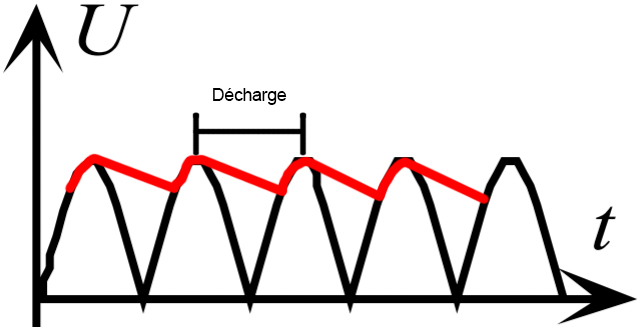
\includegraphics[scale=0.25]{Condensateur}
\columnbreak
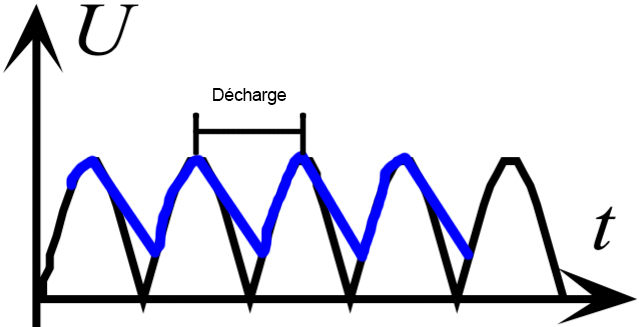
\includegraphics[scale=0.25]{Condensateur2}
\end{multicols}
A droite le courant appelé est plus important qu'a gauche, la régulation est moins bonne.
\item en prenant un condensateur de 10$\mu$F, on remarque de la sortie est beaucoup moins stable (V$\in$[1V;10V]) qu'avec le condensateur de 1000$\mu$F que nous utilisons. Notre interprétation semble être correcte.
\end{enumerate}
\section{RÉGULATION PAR DIODE ZENER SIMPLE}
Nous allons à présent tenter d'améliorer la régulation en ajoutant une diode Zener et une résistance à la suite du montage précédent.
\begin{figure}[h]
\centering
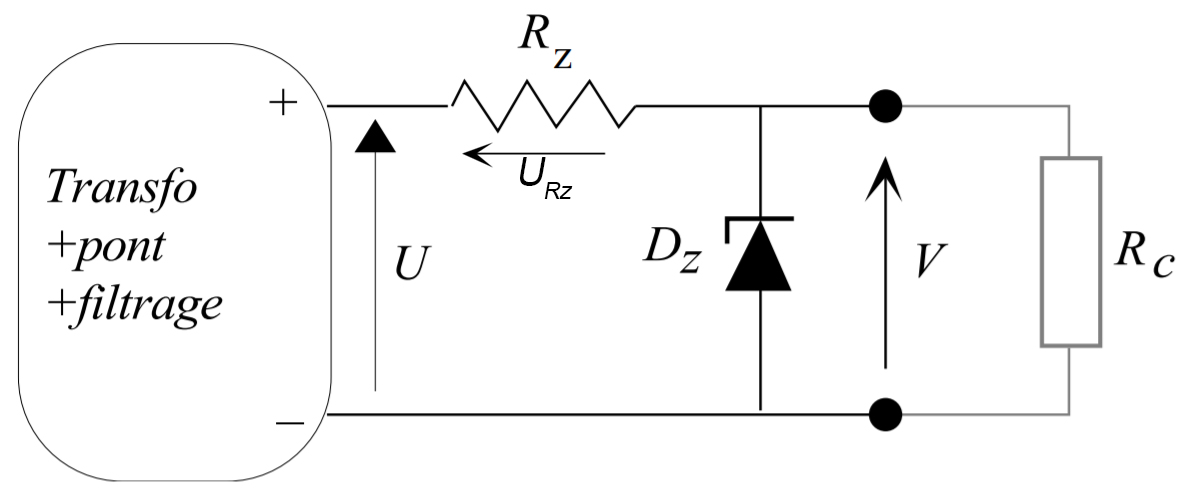
\includegraphics[scale=0.2]{Zener}
\caption[Montage avec diode Zener]{Montage avec diode Zener}
\label{fig:zener}
\end{figure}
Avant toute chose, nous devons faire attention à ne pas dissiper plus de 0,5W dans la diode Zener et plus de 0,25W dans la résistance R$_{z}$. On étudie le cas limite, i.e R$_{c}$=$\infty$, tout le courant va dans la Diode.
%\begin{multicols}{2}
\[
\begin{aligned}
\begin{cases}
P_{z}=V.I_{tot}\\
R_{z}=\dfrac{(U-V)}{I_{tot}}
\end{cases}
\end{aligned}
\iff
\begin{aligned}
\begin{cases}
I_{tot}=\dfrac{P_{z}}{V}\\
R_{z}=\dfrac{(U-V)V}{P_{z}}
\end{cases}
\implies R_{z}=\dfrac{(10-8,2)8,2}{0,5}=30\Omega
\end{aligned}
\]
Il faut donc R$_{z}$>30$\Omega$ pour ne pas dissiper plus de 0,5W dans la diode Zener. Mais comment faut-il choisir R$_{z}$ pour qu'elle ne grille pas (P$_{R_{z}}$<0,25W)?

\begin{align*}
P_{R_{z}}&<0,25W\\ \iff \dfrac{(U_{Rz})^{2}}{R_{z}}&<0,25W \iff \dfrac{(U-V)^{2}}{R_{z}}<0,25W\\
\iff R_{z}&>4.(U-V)^{2}\\
\implies R_{z}&>4.(10-8,2)^{2}=13\Omega
\end{align*}
Il faut que : 
\[
\begin{cases}
R_{z}>30\Omega\\
R_{z}>13\Omega
\end{cases}
\implies R_{z}>30\Omega
\]
Dans notre cas nous resterons largement au dessus de 30$\Omega$

\begin{enumerate}

\item Point de fonctionnement\\
Le point de fonctionnement d'un circuit est le point $(I_f,U_f)$ pour lequel le générateur et le récepteur du circuit coïncide. \\
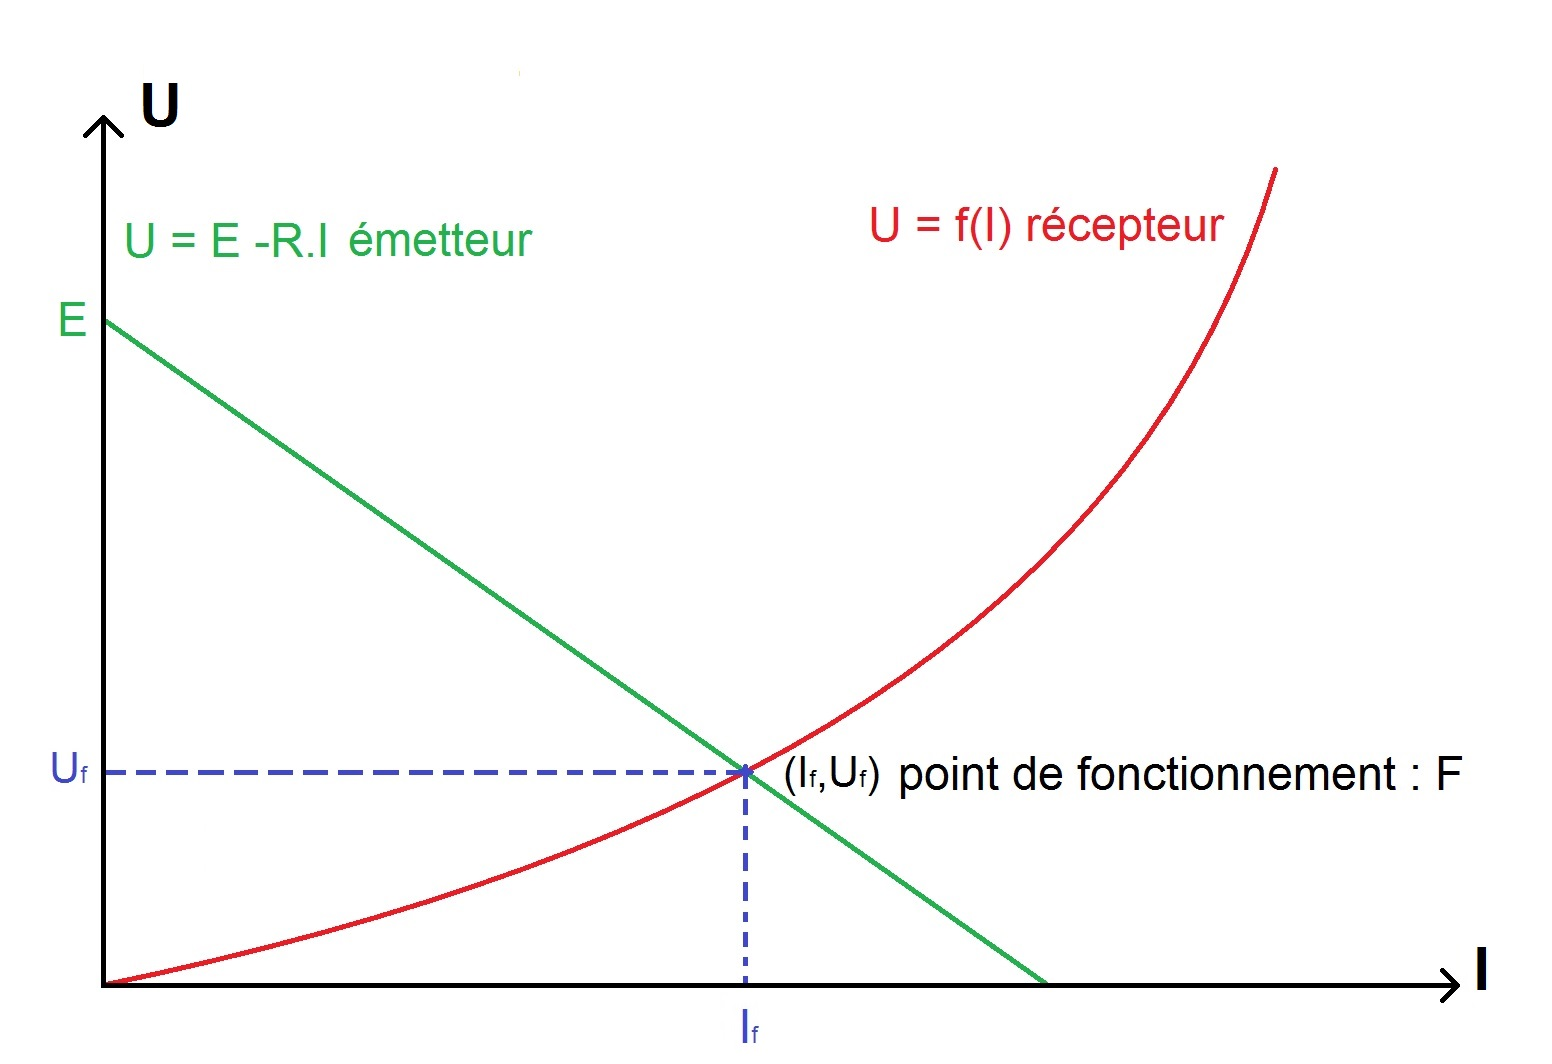
\includegraphics[scale=0.2]{imtp1}\\ 
On remarque qu'il est beaucoup plus simple de déterminer le point de fonctionnement graphiquement plutot que part calcul (les équations pouvant être compliquées) ou expérimentalement.

\item Principe de la diode zener \\
La diode zener est une diode qui par définition possède un sens unique (le courant ne peut pas faire d'aller-retour) qui a la propriétés de fonctionner qu'à partir d'une tension précise que l'on note $U_z$. Elle permet ainsi de limiter les valeurs de fonctionnement du système.\\
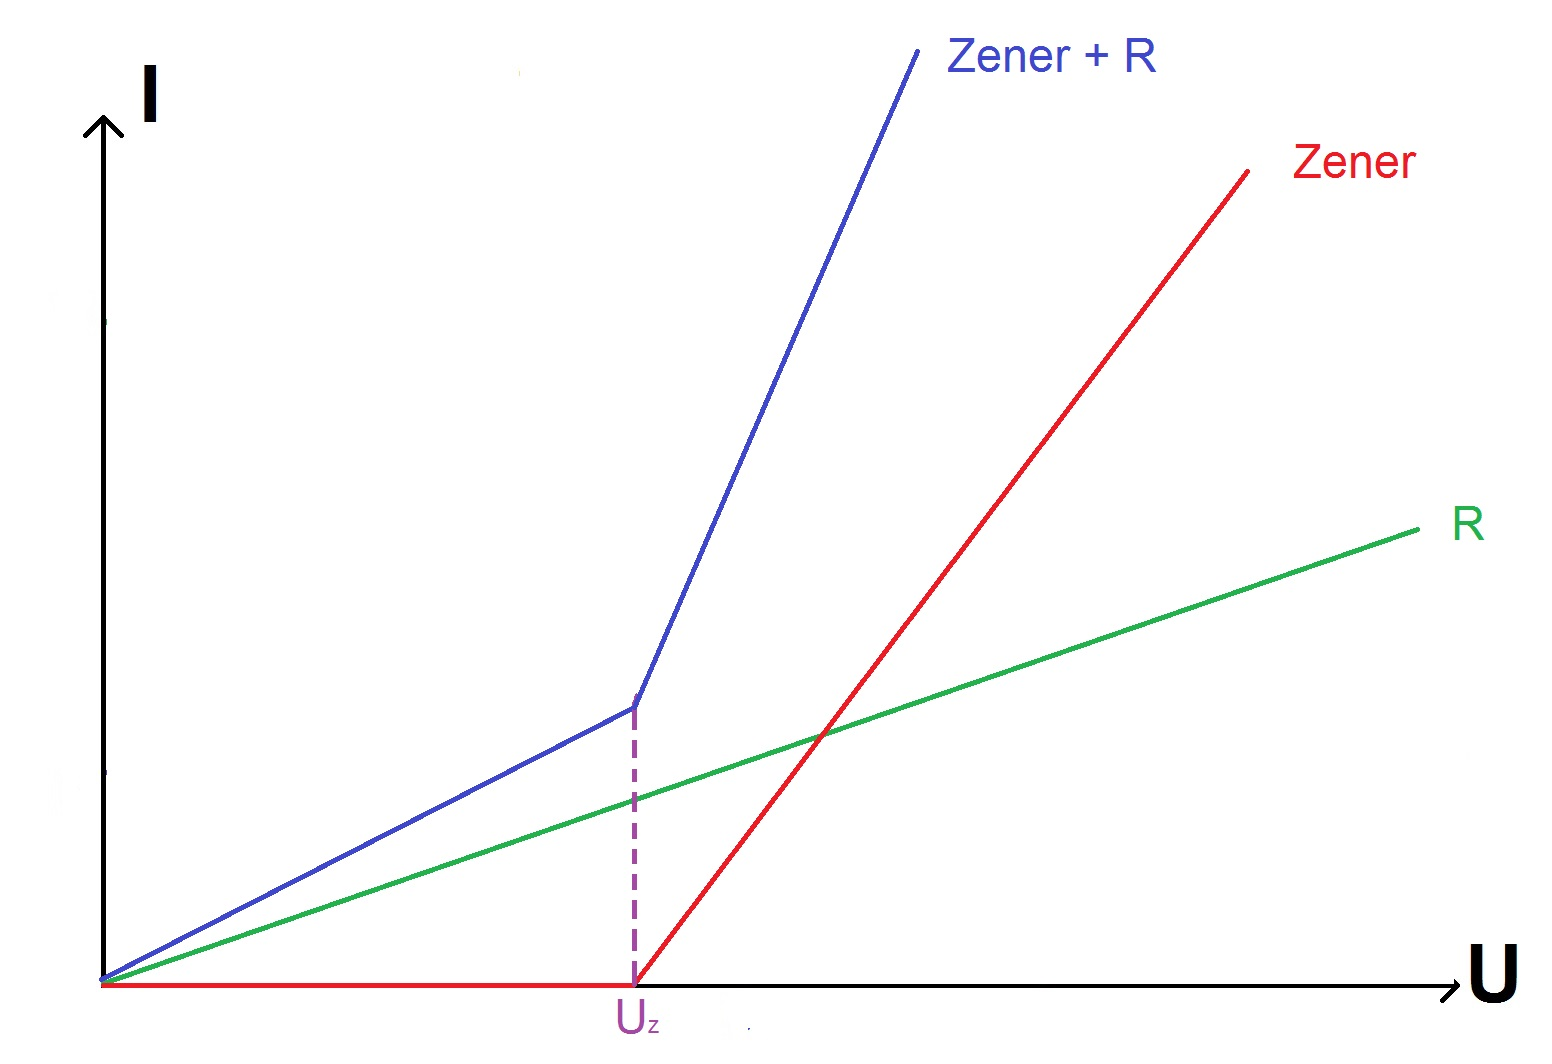
\includegraphics[scale=0.2]{imtp2}\\
La diode permet un "claquage" du courant à partir de sa tension propre $U_z$. En la combinant au circuit précédent on obtient alors une meilleur linéarité de notre régulation comme le montre le tableau suivant :\\
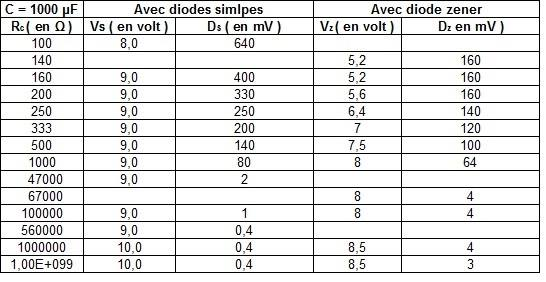
\includegraphics[scale=0.7]{tab1}\\
Avec $R_z$ = 100 $\Omega$ et $U_z$ = 8.2 V\\
On remarque que notre régulation "tombe" à partir du même ordre de grandeur de $R_c \approx 1000$  $\Omega$ et qu'avec la diode zener la décharge $D_z$ est plus faible que sans celle-ci.
\begin{bigcenter}
\begin{tikzpicture}
\begin{axis}[
height=8cm,width=16cm
,axis x line=bottom,axis y line=left
,xmin=0,xmax=6.4896
,ymin=0,ymax=86.528
,grid=major
,title={Taux d'ondulation T en fonction de $\log{(R_{c})}$}
,xlabel={logRc}
,ylabel={T/$10^{-3}$}
,legend entries={Sans diode Zener,Avec}
]
\addplot[draw=red
,smooth
,error bars/.cd,y dir=both, y explicit,x dir=both, x explicit,error mark=none
] table[x error index=2,y error index=3]
 {Tauxd'ondulation10.txt};
\addplot[draw=blue
,smooth
,error bars/.cd,y dir=both, y explicit,x dir=both, x explicit,error mark=none
] table[x error index=2,y error index=3]
 {Tauxd'ondulation12.txt};
\end{axis}
\end{tikzpicture}
\end{bigcenter}
On remarque que la diode Zener réduit le taux d'ondulation pour le faible valeur de R$_{c}$ mais augmente T si R$_{c}=\infty$ (T=3,5.$10^{-4}$ avec et T=4.$10^{-5}$ sans).
\item Choix de $R_c$\\
Pour choisir la valeur de $R_c$, en plus de tenir compte de la puissance maximale que peuvent capter la résistance et la diode zener, il a fallu tenir en compte du graphique suivant: \\
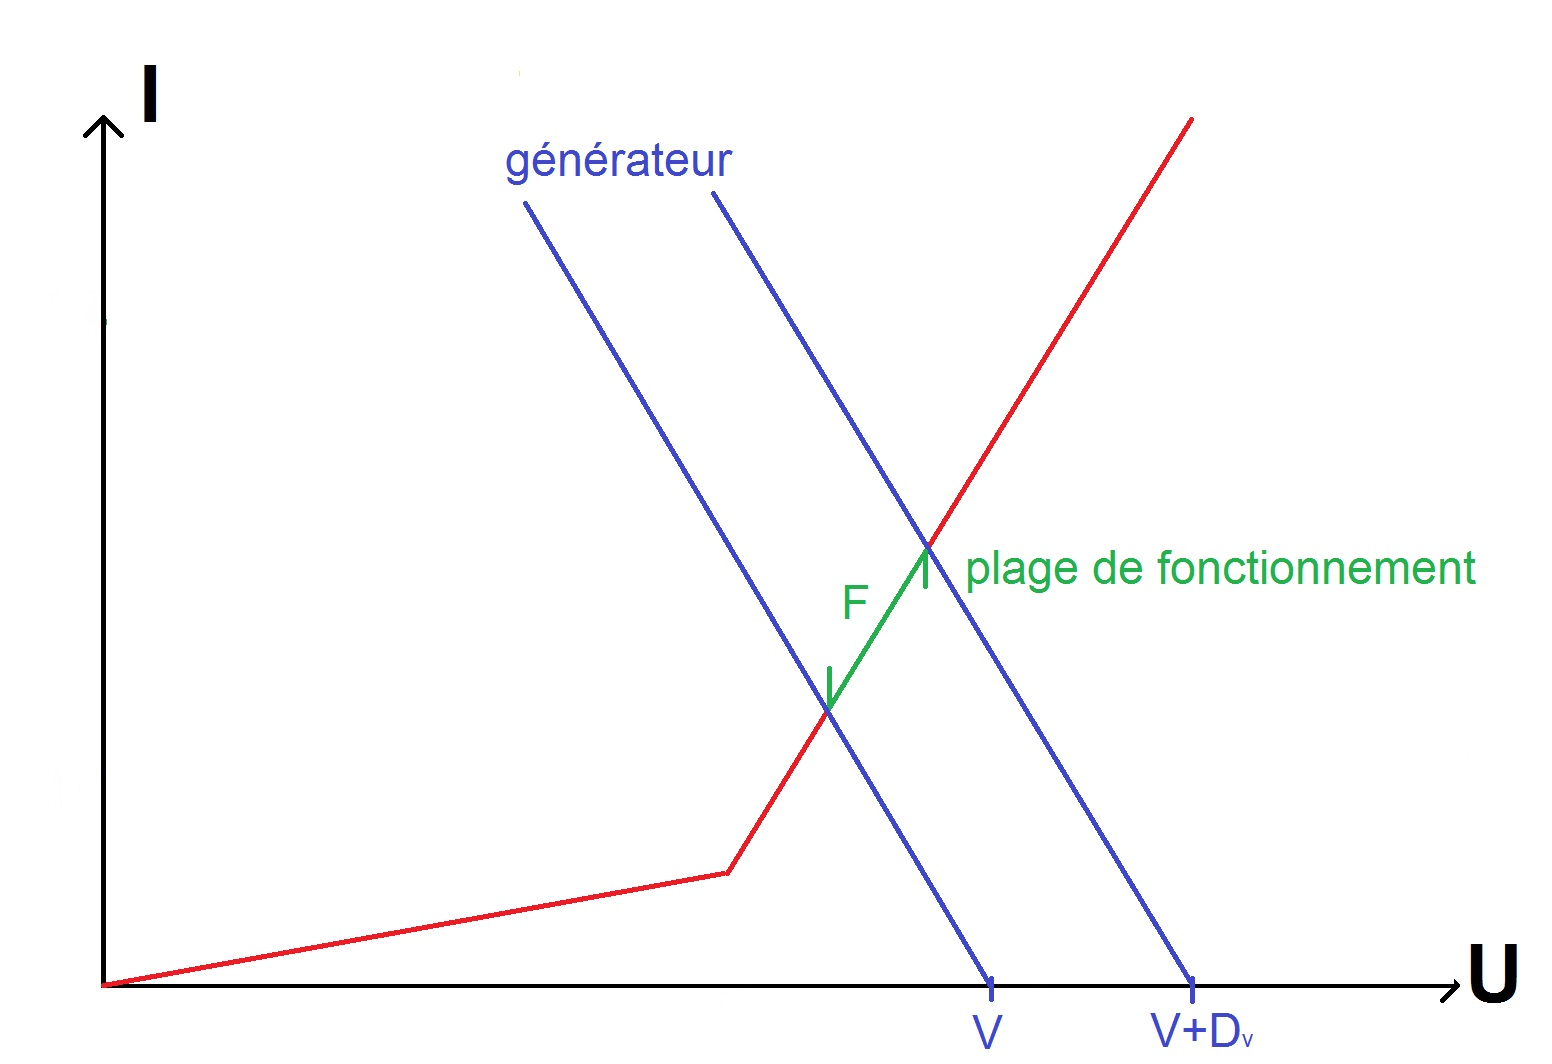
\includegraphics[scale=0.2]{imtp3}\\
Plus notre résistance est grande, plus le rapport $\frac{1}{R_c}$ est faible. Par conséquent notre montage fonctionnerait en dehors de la plage de fonctionnement de la diode zener. Il nous fallait donc une résistance faible mais pas trop.

\end{enumerate}
\end{document}
